\chapter{Design choices for better multilingual tokenizers}
\label{chap:experiment_2_properties}

% \textbf{Q3:} What is the reason that the standard tokenizer training method does not work well in the multilingual setting? 

% motivation
In this chapter, we propose and conduct a series of experiments to answer (\textbf{Q3}) what is the reason that the standard tokenizer training method does not work well in the multilingual setting.
Our goal is to explore why was the Unigram algorithm found to be unsuitable for multilingual tokenization by our related work. Moreover, we investigate the reason behind the large difference in the quality of tokenizers in the previous \autoref{chap:experiment_1_validity}.
%  \tomasz{Based on the results it's not only Unigram you explore here. So mention also BPE or subword tokenization in general.}

% overview
To answer the question, we first investigate the differences in implementation between Huggingface Tokenizers\footnote{\href{https://github.com/huggingface/tokenizers}{https://github.com/huggingface/tokenizers}} and the original Sentencepiece\footnote{\href{https://github.com/google/sentencepiece}{https://github.com/google/sentencepiece}}. Next, we look at the influence of the training data size, the alphabet size, and finally the language imbalance in the training data. In the last experiment, we will examine closely the effect of the data imbalance on the tokenizer's quality per language.

% method
\section{Experiments}

As shown in the previous \autoref{chap:experiment_1_validity}, we observe that the Huggingface Unigram tokenizer leads to significantly worse metrics than the other tokenizers.
 We investigate this difference by turning to the original Sentencepiece implementation of the algorithm and running a comparable experiment.
 For comparison, we also train a comparable BPE tokenizer using the Sentencepiece library. We evaluate the tokenizers using our metrics.

% We use the Sentencepiece library \cite{kudo_sentencepiece_2018} to train the Unigram and BPE tokenizers. We use the same hyperparameters as in the previous \autoref{chap:experiment_1_validity} for the Huggingface tokenizers. 

Next, we train a series of Unigram tokenizers on different amounts of data and see how the data amount influences the tokenizers' quality. We sample $N = 1\,000, 10\,000, 100\,000, 1\,000\,000, 1\,500\,000, 2\,000\,000$ lines for each of the 20 languages, concatenate the samples and create a balanced corpora of different sizes. We then evaluate the tokenizers using our metrics.

We proceed with a similar analysis for the alphabet size. The alphabet of a tokenizer is the set of characters that are included in the vocabulary. We hypothesize, that too large alphabet size may influence the vocabulary allocation, we therefore use the character coverage parameter of the Sentencepiece library to control the alphabet size. The character coverage parameter determines, how many distinct Unicode characters are included in the vocabulary of the tokenizer. We train a series of Sentencepiece Unigram tokenizers with the character coverage parameter set to 98\%, 99.5\%, 99.95\%, 99.995\%, 99.9995\%, and 100.0\% on data sampled with $\alpha=0.3$ from CC100. 

Finally, for the data balance experiment, we train 5 tokenizers with an increasingly imbalanced corpus with $\alpha = 0.0, 0.3, 0.5, 0.7, 1.0$ sampled from the CC100 with 20 languages. \footnote{For $\alpha = 0.0, 0.3, 0.5, 0.7$ we make sure to sample at least 100k lines per language as we have found this to be important in \autoref{sec:data_size}. We note that the data imbalance for $\alpha=1.0$ is so large, that we needed to settle for 30k-70k training lines for the five least resourceful languages (ka, ur, te, mr, sw) because of memory constraints.} On one extreme we have the $\alpha=1.0$, where all data available for each language is combined. On the other, we have $\alpha=0.0$, where the data is sampled per line from each language with the same probability. We use the Sentencepiece Unigram tokenizer with the default settings. Specifically, we use the default character coverage of 99.95\%. As usual, we evaluate the tokenizers on a balanced validation set sampled from a holdout portion of the CC100 corpus. 

% \tomaszrep{Then we switch to the original Sentencepiece library, which is used in the related work we replicate}{[E]} \cite{conneau_unsupervised_2020,chung_improving_2020,zheng_allocating_2021,liang_xlm-v_2023}. 
% \tomaszrep{We see that there are differences in the implementation of the Unigram and BPE algorithms between the two libraries and that the Huggingface library yields subpar Unigram tokenizers.}
%  We further assess other factors that influence the tokenizer's quality, such as the total training data size, the size of the alphabet, and most importantly the language imbalance in the training dataset.
% The last batch of experiments becomes the main baseline we use for comparing the next experiments.\tomasz{The batch of experiments cannot become baseline. We can design experiments to compare with given baselines.}

\section{Results}
% \tomasz{Desceibe potential sources of differences between tokenizers in experiment part. Here just write the results.}
% \tomasz{Call it ``Results''}

\subsection{Choice of implementation}
\label{sec:implementation}

\begin{table}
\caption{In this table, we compare the Huggingface and Sentencepiece implementations of the Unigram and BPE algorithms. As shown, the Huggingface Unigram tokenizer is a clear outlier in terms of all metrics. We can see that this is a problem in the implementation as the corresponding Sentencepiece \textit{unigram\_alpha0.3} scores much higher. As we will explore in \ref{tab:coverage_influence}, the different alphabet size does not influence the metrics enough to explain the difference. \xxx{here I can add an experiment with the same alphabet size, to be able to skip the reference} Interestingly, we found that the BPE implementation (\textit{huggingface\_bpe\_alpha0.25}) is better in Huggingface than in Sentencepiece (\textit{bpe\_alpha0.25}).}
\label{tab:hugg_vs_sentpiece}
\begin{tabular}{lrrrrr}
\toprule
Tokenizer & Alphabet & \# UNKs & CPT & AR & JSD \\
\midrule
huggingface\_bpe\_alpha0.25 & 1000 & 14040.1 & 3.713 & 1253.7 & 0.783 \\
unigram\_alpha0.3 & 2666 & 923.5 & 3.702 & 1190.7 & 0.768 \\
bpe\_alpha0.25 & 1215 & 7235.6 & 3.666 & 1212.9 & 0.774 \\
huggingface\_unigram\_alpha0.25 & 12616 & 4.5 & 3.204 & 1010.5 & 0.745 \\
\bottomrule
\end{tabular}
\end{table}


The results are presented in \autoref{tab:hugg_vs_sentpiece}. We see that the implementation has an effect on tokenization. We compare the Sentencepiece Unigram ($\alpha$=0.25) tokenizer trained on the same data and with the same parameters (100\% alphabet coverage) as the Huggingface Unigram ($\alpha$=0.25). We see that there is a large difference between the two. The Huggingface Unigram underperforms all of our tokenizers. On the other hand, the Sentencepiece Unigram approaches the metrics of both BPE tokenizers. We further see that if we restrict the vocabulary size for the Sentencepiece Unigram (($\alpha$=0.3)), we close the gap between Unigram and BPE. 

Interestingly, we observe that the Huggingface implementation of BPE seems to be better than the Sentencepiece implementation of BPE in our experimental setup, yielding higher vocabulary allocation metrics (CPT and AR).

Because of the subpar implementation of the Unigram algorithm in the Huggingface library, we use the Sentencepiece implementation for the rest of the experiments.

\subsection{Data size}
\label{sec:data_size}

\begin{table}
\centering
\caption{We measure how much data is generally needed for the tokenizer training. We train handful of Sentencepiece Unigram tokenizers on different amounts of balanced multilingual data. We observe that after 100k-1M lines per language, the tokenizers converge to similar vocabulary allocation and overlap scores. The significance of this experiment is that we find out experimentally how much data is needed for the tokenizer training and we can use this information to make sure that we provide enough data for each language for the further experiments.}
\label{tab:data_size_influence}
\begin{tabular}{rrrrrr}
\toprule
 Lines per language &  Alphabet size &  Number of UNKs &      CPT &          AR &      JSD \\
\midrule
               1000 &           3598 &          520.35 & 3.301636 &  958.414048 & 0.765687 \\
              10000 &           4725 &          117.75 & 3.597563 & 1089.112498 & 0.765236 \\
             100000 &           5041 &           65.55 & 3.695797 & 1192.201089 & 0.767133 \\
            1000000 &           5079 &           62.60 & 3.702038 & 1204.659073 & 0.767357 \\
            1500000 &           5176 &           55.90 & 3.705119 & 1210.664835 & 0.767348 \\
            2000000 &           5180 &           56.35 & 3.705109 & 1212.489940 & 0.767327 \\
\bottomrule
\end{tabular}
\end{table}


%We are interested in how much data is needed for the tokenizer training. For this experiment, we sample the same number of lines ($1\times10^{3}, 1\times10^{4}, 1\times10^{5}, 1\times10^{6}, 1.5\times10^{6} \text{ and } 2\times10^{6} \text{ per language}$) for each language from the CC100 corpus. Then we train Sentencepiece Unigram tokenizers on different amounts of data and compare the results in \autoref{tab:data_size_influence}. 
We are interested in how much data is needed for the tokenizer training. We present the results in \autoref{tab:data_size_influence}. We see that the metrics improve with the amount of data, but the improvement stops to be substantial after 100k-1M lines per language. We use these results as a rule of thumb for the rest of the experiments and where possible, we use at least 100k but preferably 1M lines per language.

\subsection{Character coverage}
\label{sec:character_coverage}

\begin{table}
\caption{We check the tradeoff of including a large alphabet size. We train Sentencepiece Unigram tokenizers with a different target character coverage and observe the resulting alphabet size, number of UNKs and tokenizer metrics. We observe that the alphabet size grows with the coverage and the number of UNKs decreases, as expected. We observe that at both extremes of the character coverage parameter, the vocabulary allocation decreases. The results indicate that the alphabet size between 1000 and 5000 provides a good tradeoff between the number of UNKs and the allocation metrics, while including all characters in the alphabet does not come with a significant decrease in the allocation metrics (-0.05 CPT).}
\label{tab:coverage_influence}
\begin{tabular}{lrrrrr}
\toprule
Coverage & Alphabet & \# UNKs & CPT & AR & JSD \\
\midrule
98.0\% & 539 & 17386.5 & 3.631 & 1115.3 & 0.749 \\
99.5\% & 1136 & 7786.9 & 3.702 & 1173.1 & 0.765 \\
99.95\% & 2678 & 910.6 & 3.705 & 1196.7 & 0.768 \\
99.995\% & 4813 & 83.0 & 3.695 & 1188.7 & 0.769 \\
99.9995\% & 8226 & 10.2 & 3.678 & 1164.2 & 0.769 \\
100.0\% & 13658 & 1.9 & 3.650 & 1124.1 & 0.768 \\
\bottomrule
\end{tabular}
\end{table}


% Because we observe a large difference in the alphabet size between Huggingface tokenizers (implied by the use of the default trainer settings of the library), we investigate the influence of this parameter on our tokenizer metrics. 
We are also interested in the influence of the alphabet size on our metrics. As we have seen in \autoref{tab:hugg_vs_sentpiece}, large alphabet size influences the vocabulary allocation metrics.
% We train the Sentencepiece Unigram tokenizers with different character coverage (98\%, 99.5\%, 99.95\%, 99.995\%, 99.9995\%, and 100.0\%) on data sampled with $\alpha=0.3$ from CC100. 
We show the results in \autoref{tab:coverage_influence}. 
%The character coverage parameter determines, how many distinct Unicode characters are included in the vocabulary of the tokenizer. 
We see that there is a direct relationship between the character coverage, alphabet size, and the number of unknown tokens in the validation set. We also see that our metrics are not largely affected by the alphabet size, as the alphabet accounts for at most 10\% of the whole vocabulary size 120\,000. The lowest vocabulary allocation metrics are on the extremes of the character coverage parameter, where the resulting alphabet size is either very small or very large. We assume that the small alphabet size leads to a large number of unknown tokens and the tokenizer is forced to segment words containing characters outside of the alphabet, as these unknown tokens might even be characters with diacritics. In the range of 1000-5000 alphabet size, we see that the metrics are not largely affected by the alphabet size. On the other extreme, where alphabet size is large, we suspect that the alphabet starts to take up a larger portion of the vocabulary and the tokenizer has less capacity for longer tokens which we observe as a lower overall CPT and AR. We note that the observed differences are small and including all characters in the training set does not come with a large decrease in our tokenizer metrics (-0.05 CPT and -70 AR compared to 99.95\% coverage). For later experiments, we use the Sentencepiece default character coverage of 99.95\%. When comparing tokenizers with different alphabet sizes, we are aware of the fact that the metrics might be affected by the alphabet size and we take this into account when interpreting the results.

\section{Data imbalance}
\label{sec:tokenizer_training_with_data_imbalance}

\begin{table}
\caption{We train five Sentencepiece Unigram tokenizers on increasingly imbalanced multilingual dataset. We see that the macro averaged metrics decrease with the increasing imbalance, suggesting that on average, the tokenizer represents the languages less well.}
\label{tab:data_balance_metrics}
\begin{tabular}{lrrrrr}
\toprule
Tokenizer & Alphabet & \# UNKs & CPT & AR & JSD \\
\midrule
Unigram $\alpha$=0.0 & 2975 & 617.1 & 3.712 & 1212.9 & 0.767 \\
Unigram $\alpha$=0.3 & 2666 & 923.5 & 3.702 & 1190.7 & 0.768 \\
Unigram $\alpha$=0.5 & 2859 & 729.0 & 3.618 & 1143.8 & 0.769 \\
Unigram $\alpha$=0.7 & 2733 & 883.2 & 3.556 & 1107.1 & 0.770 \\
Unigram $\alpha$=1.0 & 2476 & 1286.3 & 3.442 & 1041.8 & 0.772 \\
\bottomrule
\end{tabular}
\end{table}


% In this section, we present the tokenizers that become the baselines for comparing the related works we replicate. Our experiments with the data imbalance follow the original tokenizer training recipe from XLM-R and mBERT. The method is training the tokenizers on a corpus created by combining monolingual data in different proportions. On one extreme we have the $\alpha=1.0$, where all data available for each language is combined. On the other, we have $\alpha=0.0$, where the data is sampled per line from each language with the same probability. 

% The contribution of our method is investigating how the language imbalance affects each language individually using the metrics we have proposed. Moreover, we investigate how the other proposed methods relate to all settings of $\alpha$, not only to the unbalanced settings of $\alpha=0.5 \textrm{ or } 0.7$ as is done in \citet{chung_improving_2020,zheng_allocating_2021,liang_xlm-v_2023}.

% \tomasz{Again, don't mix setup with results!}
% For the data balancing experiment, we train 5 tokenizers with a vocabulary size of 120\,000 on an increasingly imbalanced corpus with $\alpha = 0.0, 0.3, 0.5, 0.7, 1.0$ using the CC100 with 20 languages. For $\alpha = 0.0, 0.3, 0.5, 0.7$ we make sure to sample at least 100k lines per language as we have found this to be important in \autoref{sec:data_size}. We note that the data imbalance for $\alpha=1.0$ is so large, that we needed to settle for 30k-70k training lines for the five least resourceful languages (ka, ur, te, mr, sw) because of memory constraints. We use the Sentencepiece Unigram tokenizer with the default settings. Specifically, we use the default character coverage of 99.95\%. We evaluate the tokenizers on a balanced validation set sampled from a holdout portion of the CC100 corpus. 

Finally, we investigate, how the training data imbalance between high-resource and low-resource languages affects the tokenizer performance.

The results in \autoref{tab:data_balance_metrics} demonstrate a clear disparity in the quality of tokenization depending on the data balance. Training on balanced data leads to higher overall metrics than on unbalanced data \footnote{This is naturally affected by the evaluation scheme where we weight each language equally. The equal weighting is in line with our goal of improving the tokenization for all represented languages as explained in \autoref{sec:intrinsic_evaluation}}. The imbalance also affects the alphabet size as it is possible to cover 99.95\% of the characters in the training data with a smaller alphabet because of the overrepresentation of a few high-resource languages.

\begin{figure}[h]
    \centering
    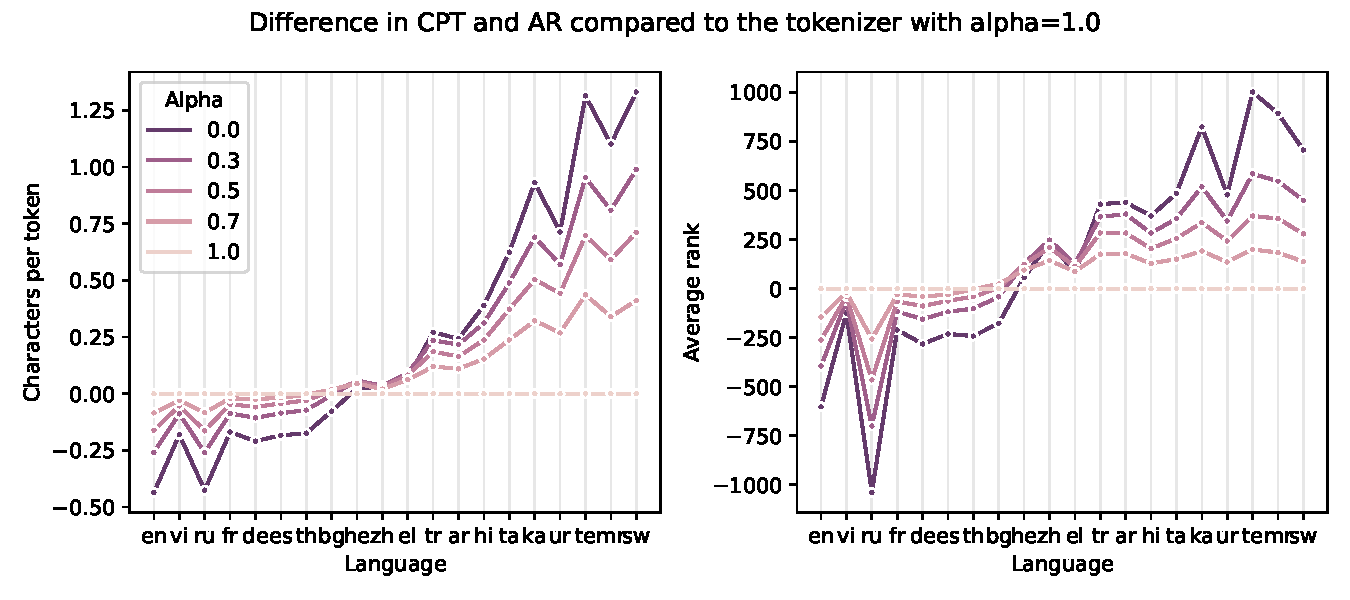
\includegraphics[width=\textwidth]{figures/ar_cpt_vs_alpha.pdf}
    \caption{We examine the impact of the language imbalance on the Sentencepiece Unigram tokenizer training. We train five tokenizers with an increasing language imbalance controlled by the $\alpha$ parameter. Then we look at the effect on the vocabulary allocation metrics per language. We subtract the results using the most unbalanced tokenizer with $\alpha=1.0$. As expected, the more balanced tokenizers have higher vocabulary allocation scores for low-resource languages and lower scores for high-resource languages. Interestingly, the effect varies across languages. For example, the vocabulary allocation of high-resource Vietnamese or French is not as affected by the decrease in training data as English or Russian.}
    \label{fig:data_balance_vs_allocation_per_lang}
\end{figure}

We explore the reason for the decreasing performance of the tokenizers trained on imbalanced data in \autoref{fig:data_balance_vs_allocation_per_lang}. We plot the differences in vocabulary allocation metrics between the most unbalanced tokenizer $\alpha=1.0$ and the rest of the tokenizers. We sort the languages by the data size available starting with the highest-resource languages and ending with the low-resource. We see that the vocabulary allocation metrics for the high-resource languages (en, vi, ru, fr, es, th) are decreasing with the increasing data balance between the languages, compared with the unbalanced baseline. On the other hand, the low-resource languages (ka, ur, te, mr, sw) are disproportionally more improved by the increasing balance and their vocabulary allocation metrics are increasing significantly. This suggests that the marginal benefit of adding more data to the high-resource languages is lower than the incurred cost on the quality of tokenization for the low-resource languages. We see the result of this tradeoff in the \autoref{tab:data_balance_metrics} as an overall decrease in the average CPT and AR.

We hypothesize, that a possible reason that the standard method of training a tokenizer on a joint corpus was reported to not work by the existing works \cite{rust_how_2021,chung_improving_2020,zheng_allocating_2021,liang_xlm-v_2023} might be the data imbalance in the training data. \citet{rust_how_2021} finds the mBERT tokenizer trained with $\alpha=0.7$ inadequate to represent low-resource languages. \citet{chung_improving_2020} and \citet{zheng_allocating_2021} use the Unigram baseline with $\alpha=0.7$. While \citet{liang_xlm-v_2023} uses a baseline with $\alpha=0.5$. All balancing methods report the most substantial improvements on the low-resource languages. In the next chapter, we will therefore compare the balancing methods with the Sentencepiece Unigram trained on balanced and unbalanced data.


\section{Findings}

In this chapter, we have investigated \textbf{Q3:} What is the reason that the standard tokenizer training method does not work well in the multilingual setting? To this end, we explore how different design choices affect the quality of the tokenizers. 

We find that the implementation of the Unigram algorithm in the Huggingface library is subpar and that the Sentencepiece implementation yields better results.

We observe that we need around 100k-1M lines per language to train a good, multilingual tokenizer. 

The alphabet size affects the number of UNK tokens but does not have a significant influence on the rest of the metrics if we stay in the range of 1000-5000 alphabet size. 

Most importantly, we observe that tokenizer training data imbalance influences the per-language metrics heavily and that it lowers the tokenization quality for the low-resource languages more than it improves it for the high-resource.